%----------------------------------------------------------------------------
\chapter{Background}
%----------------------------------------------------------------------------

In this chapter, the fundamental concepts about the graph databases and graph engines used in our thesis are discussed. We present formal definitions of the concepts based on~\cite{DBLP:journals/csur/AnglesABHRV17}.

%----------------------------------------------------------------------------
\section{Graph database models}
%----------------------------------------------------------------------------

Graphs are used to encode the data objects and relationships between them, named nodes, and edges, respectively.
For example, if a graph designed to store the movie and actor data, nodes can be actors and movies, relationships will be defined according to which actors acted in the movie.
The graph representation in \autoref{fig:graph_movie} indicates different actors have acted in one movie. Edge directions matter, \ie an edge cannot be directed from a movie into an actor node.

\begin{figure}[!ht]
  \centering
  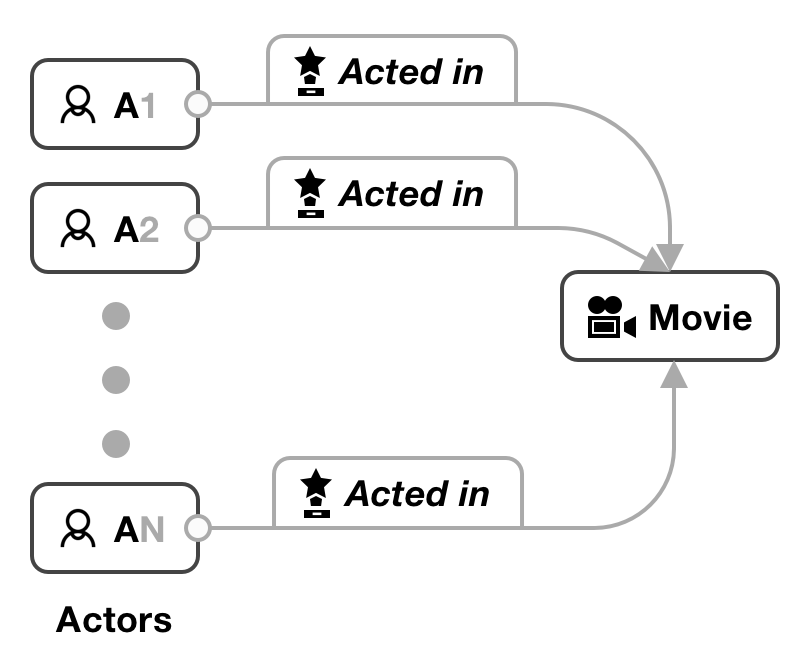
\includegraphics[scale=0.3]{figures/graph_movie.png}
  \caption{Simple movie graph. Based on~\cite{DBLP:journals/csur/AnglesABHRV17}} 
  \label{fig:graph_movie}
\end{figure}

However, it is often not possible to capture a scenario in a simple graph.
For example, an actor can be a director of the movie at the same time.
In this case, we need to introduce multiple edges between nodes to define these relationships (\autoref{fig:graph_movie_different_edges}).

\begin{figure}[!ht]
  \centering
  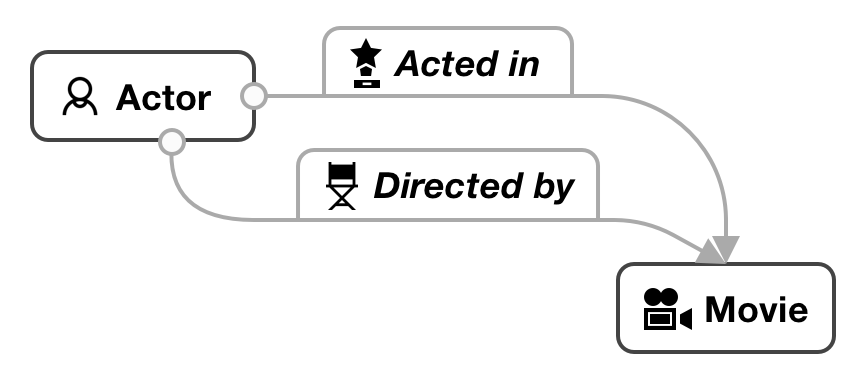
\includegraphics[scale=0.3]{figures/graph_movie_different_edges.png}
  \caption{Movie graph with multiple type edges. Based on~\cite{DBLP:journals/csur/AnglesABHRV17}} 
  \label{fig:graph_movie_different_edges}
\end{figure}

The remaining problem is the identification of nodes. To this end, labels and properties are used, allowing precise lookups in graphs.

\subsection{Edge-labelled graphs} 

The labels are assigned to different types of relationships in order to handle the multi-edge identification problem.
It is a simple and widely used method in graph setups.
In \autoref{fig:graph_movie_different_edges} we have two edge types, namely \textsf{Acted in} and \textsf{Directed by}.

\begin{definition}\label{def:edge_labelled_graph}\cite{DBLP:journals/csur/AnglesABHRV17}
An edge-labelled graph G is a pair (\textit{V, E}), where:

\begin{enumerate}
  \item \textit{V} is a finite set of \textit{vertices} (or \textit{nodes}).
  \item \textit{E} is a finite set of edges; formally, \textit{$E \subseteq V \times \mathit{Lab} \times V$} where \textit{Lab} is a set of labels.
\end{enumerate}
\end{definition}

Edge-labelled graphs can express complex scenarios by introducing an additional node representing the edge.
For example, we would like to capture that one actor has been acted multiple times in the same movie.
With the previous implementation, it seems impossible to add the same labelled edge between two nodes; however, we can get this information with further granulation of the movie node.
This way, an actor can play a different role in the same movie, and relationships can be built between actor roles instead of targeting the movie itself (\autoref{fig:graph_complex_edge_labels}).
The newly introduced \textsf{Role} node can also hold additional data for further processing, such as screen time of different roles is played in the movie by one actor.

\begin{figure}[!ht]
  \centering
  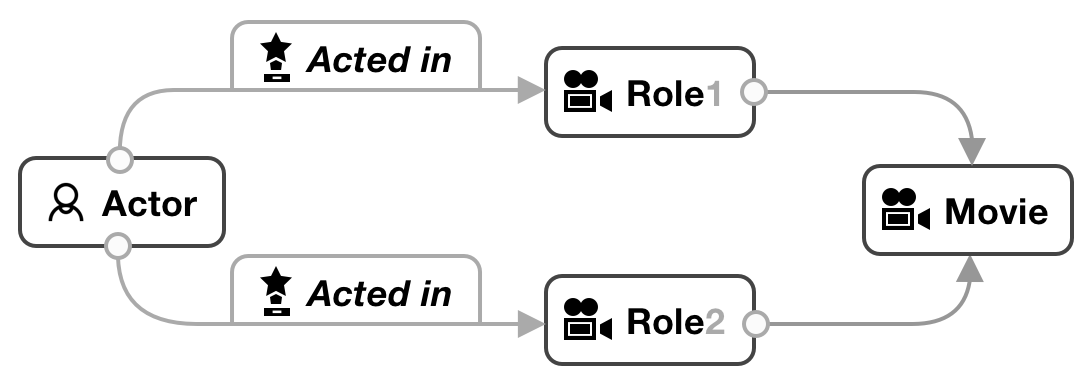
\includegraphics[scale=0.3]{figures/graph_complex_edge_labels.png}
  \caption{Actor edge is connected to the same movie through multiple role nodes. Based on~\cite{DBLP:journals/csur/AnglesABHRV17}} 
  \label{fig:graph_complex_edge_labels}
\end{figure}

\subsection{Property graphs}

In edge-labelled graphs, we differentiate the edge types by their labels.
The nodes also can be labelled for this purpose.
For example, in \autoref{fig:graph_movie} the actor and movie can be labelled \textsf{User} and \textsf{Movie} respectively.
We can assign multiple labels to one node, like in \autoref{fig:graph_movie_different_edges} an actor node can be labelled as \textsf{Actor} and \textsf{Director} as well.
This kind of node labels decreases the abstraction gap between the modelled concept and their representation, and allows easier query design for users.

On the other hand, it is challenging to add more information into edges in edge-labelled graphs.
In \autoref{fig:graph_movie} if we would like to add source information to the \textsf{Acted in} edge, new edge additions would not suffice.
We need to introduce a new type of n-ary relation with information we would like to add, the fact nodes in relationship with \textsf{Acted in} edges.
Adding new types of edges and nodes into edge-labelled graphs is costly and may require more considerable structural changes.

In real-world applications, a new type of metadata additions is prevalent.
The general and widely used solution is property storage inside the edge and nodes, called a \textbf{property graph}.
This model is adopted by some modern graph database engines, Neo4j~\cite{neo4j_website}, TigerGraph~\cite{tigergraph_website}, Oracle PGX~\cite{pgx_website} are good examples and used in our experiments as well.

In property graphs, edges and nodes can be labelled, and each entry is associated with an identifier that enables the direct referencing.
In \autoref{fig:graph_properties}, the previously discussed source information for the \textsf{Acted in} edge is added as a property parameter.
The caption in the top of nodes and edges represents their label; the list underneath defines the possible properties that are held in it.
Here we get a simple data storing instead of declaring new edges and nodes to store information about the source, gender in \textsf{Acted in} edge, and \textsf{Person} node, respectively.

\begin{figure}[!ht]
  \centering
  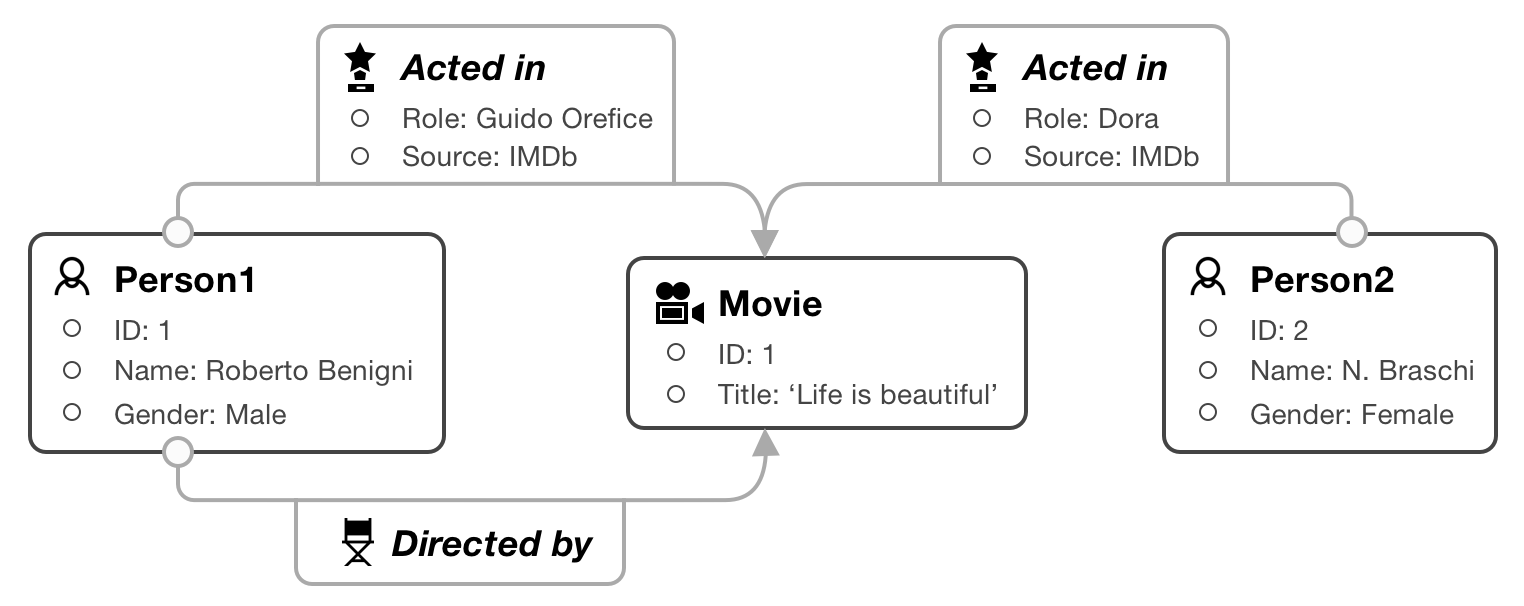
\includegraphics[scale=0.26]{figures/graph_properties.png}
  \caption{Property graph of movie database elements. Based on~\cite{DBLP:journals/csur/AnglesABHRV17}} 
  \label{fig:graph_properties}
\end{figure}

\begin{definition}\label{def:property_graph}\cite{DBLP:journals/csur/AnglesABHRV17}
A property graph $G$ is a tuple (\textit{$V, E, \rho, \lambda, \sigma$}), where:

\begin{enumerate}
  \item $V$ is a finite set of vertices (or nodes).
  \item $E$ is a finite set of edges such that $V$ and $E$ have no elements in common.
  \item $\rho$ : $E \rightarrow (V \times V)$ is a total function. Intuitively, $\rho(e) = (v_1, v_2)$ indicates that $e$ is a directed
  edge from node $v_1$ to node $v_2$ in $G$.
  \item $\lambda$ : $(V \cup E) \rightarrow Lab$ is a total function with $\textit{Lab}$ a set of labels. Intuitively, if $v \in V$ (respectively, $e \in E$) and $\rho(v) = \ell$ (respectively, $\rho(e) = \ell$) , then $\ell$ is the label of node $v$ (respectively, edge $\ell$) in $G$.
  \item $\sigma$ : $(V \cup E) \times \textit{Prop} \rightarrow \textit{Val}$ is a partial function with $\textit{Prop}$ a finite set of properties and $\textit{Val}$
  a set of values. Intuitively, if $v \in V$ (respectively, $e \in E)$, $p \in \textit{Prop}$ and $\sigma (v,p) = s$ (respectively, $\sigma (e,p) = s$), then $s$ is the value of property $p$ for node $v$ (respectively, edge $e$) in the
  property graph $G$.
\end{enumerate}
\end{definition}

%----------------------------------------------------------------------------
\section{Graph patterns}
%----------------------------------------------------------------------------

Several functional and declarative query languages have been introduced in the last decade to handle the graph data models we discussed in the previous chapter.
The earliest and multi-vendor adopted query language was SPARQL\footnote{\url{https://www.w3.org/TR/rdf-sparql-query/}}, the query language for RDF.
It was initially standardized by the W3C in 2008 and upgraded to 1.1 in 2013.
For the sake of other popular query languages for property graphs, Cypher\footnote{\url{https://neo4j.com/developer/cypher-basics-i/}} and Gremlin\footnote{\url{https://tinkerpop.apache.org/}} are good examples and are used in the Neo4j and Apache TinkerPop engines respectively.

However, these languages are working with different technologies, computation methods, they share a common conceptual core of querying graphs.
There are two types of essential operations in the context of querying graphs:

\begin{enumerate}
  \item Graph pattern matching
  \item Graph navigation
\end{enumerate}

The simplest form of the graph pattern matching is searching for matches of a graph-structured query in the graph database.
In the more complex scenario, these patterns can be augmented with other features, like projection, union, optional, and difference.
With the help of additional features, we get more detailed and refined subgraph results.
Pattern matching in a graph is a core conceptual core of SPARQL, Cypher, and Gremlin.
They are used in different practical applications, such as pattern recognition, machine learning, planning, fraud detection, and more.

\subsection{Basic graph patterns}

The core principle of the graph database queries is basic pattern matching.
Basic graph patterns look for the same subgraph structure in the database in the simplest form, additionally with predefined condition variables.
For example, variables in the edge-labelled graphs can be described with nodes and edge labels, in property graphs with any constants.
Property graphs can be queried with the label and different types of property variables. 
In summary, basic graph patterns map the query variables to the database constants to find the exact matches.

\begin{definition}\label{def:basic_graph_patterns}\cite{DBLP:journals/csur/AnglesABHRV17}
More formally, let us refer collectively to the sets of terms $V$ and $\textit{Lab}$ from Definition~\ref{def:edge_labelled_graph} and the sets of terms $V$ , $E$, $\textit{Lab}$, $\textit{Prop}$, and $\textit{Val}$ from Definition~\ref{def:property_graph} as $\textit{constants}$, 
denoted $\textit{Const}$. Let $Var$ denote a set of $\textit{variables}$. We could then define basic graph patterns (bgps) for graph databases in relation
to Definition~\ref{def:edge_labelled_graph} by allowing $V$ and $\textit{Lab}$ to contain $\textit{variables}$, and likewise we could define bgps for
property graphs in relation to Definition~\ref{def:property_graph} by allowing $V$, $E$, $\textit{Lab}$, $\textit{Prop}$, and $\textit{Val}$ to contain variables.
\end{definition}

The basic graph pattern query ($Q$) computes all possible matches of $Q$ in a graph database $G$.

\begin{definition}[Match]\label{def:match}\cite{DBLP:journals/csur/AnglesABHRV17}
Given an edge-labelled graph $G = (V, E)$ and a \textit{bgp} $Q = (V', E')$, a match $h$ of $Q$ in $G$ is a mapping from $\textit{Const} \cup \textit{Var}$ to $\textit{Const}$ such that:

\begin{enumerate}
  \item for each constant $a \in \textit{Const}$, it is the case that $h(a) = a$; that is, the mapping maps constants
  to themselves
  \item for each edge $(b,l,c) \in E$, it holds that $(h(b),h(l),h(c)) \in E$; this condition imposes that
  ($a$) each edge of $Q$ is mapped to an edge of $G$, and ($b$) the structure of $Q$ is preserved in its
  image under $h$ in $G$ (that is, when $h$ is applied to all the terms in $Q$, the result is a sub-graph
  of $G$).
\end{enumerate}
\end{definition}

\subsection{Complex graph patterns}

In the basic relational operations, previously discussed basic graph patterns cover the natural join and equality based matching.
In the complex graph patterns matching conditions are extended with operations like projection, union, difference, optional (also known as  left-outer-join), and filter.
We will discuss each operation separately in the following.

\paragraph{Projection}

In the bgp \textit{Q(G)} we expect to return all the matched subgraphs with the full set of parameters in the \textit{output variables}.
However, in some cases, we focus the only subsection of output variables in a graph pattern matching.
For example we are getting an output result from the movie graph database with actor details, \textsf{name}, \textsf{surname}, \textsf{gender}, \textsf{birthdate}, \textsf{oscarAwarded}, but in the data processing side only two of them, \textsf{name} and \textsf{surname}, are required.
In the cgp queries, it is possible to add extra output pipeline and get a \textbf{projection} of full output.
This operator is widely common in all graph database engines, often used with keyword \texttt{SELECT} as used by \textmd{SQL}.

\paragraph{Join}

Multiple bgp outputs can be joined quickly with another bgp, but more complex patterns with different semantics require explicit use of this operator.
This behavior is achieved usually over a natural join between two graph patterns $Q_1$ and $Q_2$. 
The common output variables of the join operation are the union of output variables of $Q_1$ and $Q_2$.
The evaluated output contains the matches by joining the matching evaluation by $Q_1$ with all matches of $Q_2$.
Respectively, two matches can be joined if the output variables of queries share their variable values, meaning that these matches are compatible.
An explicit join operator is used in query languages where complex matching results are needed to be combined from different operations.

\paragraph{Union and difference}

The union of graph patterns $Q_1$ and $Q_2$ is a complex pattern, necessitating computing the union of $Q_1$ and $Q_2$ evaluations.
For example, in the movie database scenario, we can build a pattern matching query to find movies where actor $A$ is acted or directed with using the union operator.
The difference of graph patterns $Q_1$ and $Q_2$ is also a complex graph pattern which requires computing the difference of $Q_1$ and $Q_2$ evaluations.
In the movie database example, we can build such a complex query to find movies where actor $A$ acted, but not directed by them using the difference operator.
The union operation evaluation is simpler than difference evaluation in computation complexity medium; as a result, most systems implement this operators
Due to the complexity of the difference operator, it is often not included in early releases of language, like in SPARQL's case, where an explicit difference operator, called \texttt{MINUS}, was only introduced in SPARQL~1.1.

\paragraph{Optional}

This operator does a similar job with the join of two patters $Q_1$ and $Q_2$, but it does not limit the $Q_1$ results matching with $Q_2$ evaluation.
The final output of this operator is a union of two pattern outputs independently.
This operator is useful to retrieve maximum information from the graph where constraints are incomplete, or data is not formatted.
For example, a client wants to query the social network graph database where users follow the celebrity $C_1$ and retrieve the average age over incomplete column \textit{birthdate}.
With the natural join operator, we will only get the results where \textit{birthdate} field exists, but the client would like to see the full list.
In this case, using \textbf{optional} operator query will return all users with the missing fields left blank.
The optional operator is called \textit{left-outer join} in relational terms and is supported most of the modern systems, including SPARQL and Cypher.

\paragraph{Filter}

Complex graph pattern queries can be used to limit the matching series by introducing intermediate values return by inequalities or their type of boolean expressions.
For example, a user wants to query the movie graph database for actors aged between 40 and 60.
To build a cgp query for this specification, we can apply filter operator over the \textit{birthdate} parameter in the following form:

\begin{lstlisting}[language=Cypher,frame=single,caption={Filtering over the birthdate parameter in Cypher}]
MATCH (a:Actor)
WHERE a.birthDate > 01.01.1960 AND a.birthdate < 01.01.1980
RETURN a
\end{lstlisting}

The filter operator does not change the output variables, only limits the result to a subset.
Filter expressions can be built with the typical conditions permitted by the selection relation operator, such as inequalities with boolean operators \textit{AND}, \textit{OR}, \textit{NOT}.
In modern query languages, a wide variety of complex filtering expressions are supported, including regular expressions over strings, arithmetic operators, casting, and datetime support.

%----------------------------------------------------------------------------
\section{Navigational queries}
%----------------------------------------------------------------------------

As graph patterns allow us to query the database within bounded constraints, the real-world graph problems are also required for finding data over navigation edges.
One of the popular query examples is the \textit{n-hop} pattern in a social network; for example, in the 2-hop pattern, we can find all friends-of-a-friend of the specified person. 
This kind of query requires navigation through the graph using a path, so they are called path queries.
Path queries are at the core of the navigational graph querying area and supported by most of the modern graph engines, including Neo4j~\cite{neo4j_website}, TigerGraph~\cite{tigergraph_website}, and Oracle PGX~\cite{pgx_website}.

\subsection{Path queries}

The most basic navigational objects in the graph database are paths.
In the basic usage, the query will look for the existence of a directed path between two nodes in a property graph without considering edge labels.
Path queries are at the core of reachability and transitive closure problems in directed graphs and well studied by the research community.
However, in practice, path queries are mainly constrained with edge labels.
As we discussed previously, the \textit{n-hop} pattern in the social network depends on the paths where \textsf{Knows} edge types exist between two person nodes.


\begin{definition}\label{def:path_query}\cite{DBLP:journals/csur/AnglesABHRV17}

We can formulate the patch query with $P = x \xrightarrow{\alpha} y$, where $\alpha$ defines the conditions on the path, $x$ and $y$ are the endpoints of the paths.
$x$ and $y$ can be denoted with variables, specified nodes, or even the same nodes if we are looking for a cyclic path pattern.
To express the $\alpha$, we can use $*$ for non-constrained queries -- the existence of the path is enough.
For more complex path queries $\alpha$ can describe regular expressions that allow for concatenating paths, applying a union/disjunction of paths, and applying a path zero or many times.
  
\end{definition}

For example in \autoref{eq:path_query_expression}, symbol "$+$" denotes the "one-or-more" \textsf{knows} edge occurrence. 
The "$\cdot$" and $|$ symbols represent a concatenation and union operators respectively.
So $x$ should know and have either a \textsf{likes} or a \textsf{dislikes} relationship with $y$ node. 

\begin{equation}\label{eq:path_query_expression}
P := x \xrightarrow{\text{knows}^+\cdot\text{(likes|dislikes)}} y
\end{equation} 

We can use an \textit{inverse} operator in path expressions to specify the traversal of edges in a backwards direction.
In the query in \autoref{eq:path_query_expression_inverse}, $x$ denotes the actor node and $y$ movie node in the movie graph.
The first \textsf{actedIn} edge lists movies $y$ where actor $x$ is acted in and following negative operator changes the navigation towards the actor node $x$.
This query will return a list of co-star actors in relative to actor $x$.

\begin{equation}\label{eq:path_query_expression_inverse}
P := x \xrightarrow{(\text{actedIn}\cdot\text{actedIn}^-)^+} y
\end{equation} 

\paragraph{Evaluation}

In the graph patterns, there are different practical considerations, \eg cyclic edge patterns need to set semantics (as opposed to bag semantics) for efficient evaluation.
Semantics help the algorithm of $P$ to decide which paths are included in $P(G)$.
We will discuss the most common evaluation forms in practice:

\begin{enumerate}
  \item \textbf{Arbitrary path semantics}
  In this type, all paths are evaluated as accepted paths in $G$ that satisfy the constraints of query $P$.
  User needs to pay extra attention under this semantics, not all the problems are feasible to enumerate the cyclic paths.
  The existence of the pattern or infinite pairs of nodes connection over such paths can be practical to use such semantics.
  \item \textbf{Shortest path semantics}
  In this type, the engine will compare and choose the shortest paths that satisfy with defined minimal length constraint by $P$.
  In practice, we can use this semantics to find pairs of nodes that have linked paths with minimal path length.
  For example, friend recommendation systems are working with the same criteria.
  \item \textbf{No-repeated-node semantics}
  In this type, the query will find the matching paths where each node is included once.
  This kind of path is called \textit{simple paths} and widely used in practical problems.
  Route finding is a good example, where it is not desirable to pass the same place more than once.
  \item \textbf{No-repeated-edge semantics}
  This type is similar to the previous one, $P(G)$ will return the matching paths where each edge has appeared once.
  In practice, this semantics also suitable for the route-finding problem.
  In this case, the same places will be desired to travel more than once but through different routes.
\end{enumerate}

The user may have different expectations from the evaluation of $P(G)$, such as: 
What is the shortest path to get some destination?
Does the graph have such a pattern path? 
What are the paths of $P(G)$?
We can categorize the output types of navigational queries:

\renewcommand{\labelitemi}{\textendash}
\begin{itemize}
  \item \textit{Boolean:}
  In the simplest output case, we need to get a validation from the graph if the query is true/false.
  In practice, the $P(G)$ can evaluate whether it is non-empty, or path pattern exists in the $G$ between defined nodes.
  \item \textit{Nodes:}
  In some applications $P(G)$ is expected to return all node pairs connected by a specific path.
  \item \textit{Paths:}
  In this case, we are interested in getting the full paths from $P(G)$.
  Like we discussed previously, in the route-finding problem, a shortest-path semantics can be applied and return the matching route paths based on custom constraints.
  The route paths can be sorted by time, weather, transport dependent variables to get some top-$k$ ``best'' paths.
  \item \textit{Graphs:}
  This type of output is mostly used under arbitrary path semantics, where the user is interested in a compact representation of graphs; for example, evaluated paths construct a new subgraph.
\end{itemize}

%----------------------------------------------------------------------------
\section{Graph database engines}
%----------------------------------------------------------------------------

We used three modern graph database engines in our work: Neo4j, TigerGraph, and Oracle PGX.
In this section, we will discuss their main properties in detail to deliver the fundamental knowledge before our graph implementations.

\subsection{Neo4j}

Neo4j is an open-source NoSQL graph database engine written in Java and Scala.
It is ranked as the first place among other graph database technologies\footnote{\url{https://db-engines.com/en/ranking/graph+dbms} (May 2020)}.
Neo4j provides cluster support, ACID transaction support, high availability, and fast query speed through traversals.
It can handle billions of nodes and relationships with acceptable computational performance.
Providing rich documentation and having a big community is among the advantages of Neo4j products.
In the following list, the main properties of the Neo4j database management system will be discussed~\cite{neo4j_website}:

\renewcommand{\labelitemi}{\textendash}
 \renewcommand\labelitemii{\textbullet}
\begin{itemize}
  \item \textbf{Data model:}
  Neo4j database works with the property graph model, nodes and edges can contain additional information in key-value pairs (called properties).
  The database supports a flexible schema, any property can added and removed (which is typical in NoSQL systems).
  \item \textbf{ACID properties:}
  It supports full ACID rules:
    \begin{itemize}
      \item Atomicity
      \item Consistency
      \item Isolation
      \item Durability
    \end{itemize}
  \item \textbf{Scalability and reliability:}
  The database can be scaled easily without affecting the query processing performance and data integrity.
  Data can be replicated for redundancy purposes to increase the safety and reliability.
  \item \textbf{The traversal of the graph:}
  Traversal operation is a navigation action in graph nodes starting with defined node and navigates through connected edges.
  Traversal action eliminates the costly full graph queries and reaches the required node with connected paths.
  \item \textbf{Built-in web application:}
  Neo4j provides a user-friendly web application, can be connected to a local or remote database over TCP or Bolt connector\footnote{\url{https://neo4j.com/docs/operations-manual/current/configuration/connectors/}}.  
  Using web application user can monitor the database, write Cypher queries and get interactive graphical output.
  \item \textbf{API:}
  Developers can manipulate the database over several mediums:
    \begin{itemize}
      \item REST API
      \item Javascript
      \item Cypher API (Java)
      \item Native Java API
    \end{itemize}
  \item \textbf{Indexing:}
  Neo4j supports indexing for more efficient search lookup.
  With Cypher user can create indexes based on one or more properties for all nodes, called \textit{single-property index} and \textit{composite index}, respectively.
\end{itemize}

\paragraph{Cypher}

Cypher is a declarative graph language developed by Neo4j and used to express efficient queries, update and manipulate the graph\footnote{\url{https://neo4j.com/docs/cypher-manual/current/introduction/}}.
It has an intuitive structure, can be understandable even by reading commands natively by regular people.
Cypher is designed to be simple and usable for users to focus on the business logic instead of getting lost in the documentation. 

Most of the Cypher commands are inspired by well-known technologies, \eg \texttt{WHERE} and \texttt{ORDER BY} are taken from SQL.
The pattern matching style is similar to SPARQL's.
Some of the semantics are borrowed from general-purpose programming languages, like Haskell and Python.
Cypher syntax is close to the English language, which makes queries easy to write and to read.

Cypher queries are structured in several clauses, like in SQL.
Clauses are chained together, and pass the result in a waterfall fashion.
For example, \texttt{MATCH} clause will pass the matched results context based on its filtering criteria, and the next clause will accept it.

The most commonly used clauses in simple queries:

\begin{itemize}
  \item \texttt{MATCH}: 
  In this clause, a graph pattern is evaluated and all matches are passed to the following clause.
  \item \texttt{WHERE}:
  This clause adds constraints to pattern or filters intermediate results passing through \texttt{WITH}.
  \item \texttt{RETURN}:
  Returns the final result.
\end{itemize}

\begin{figure}[!ht]
  \centering
  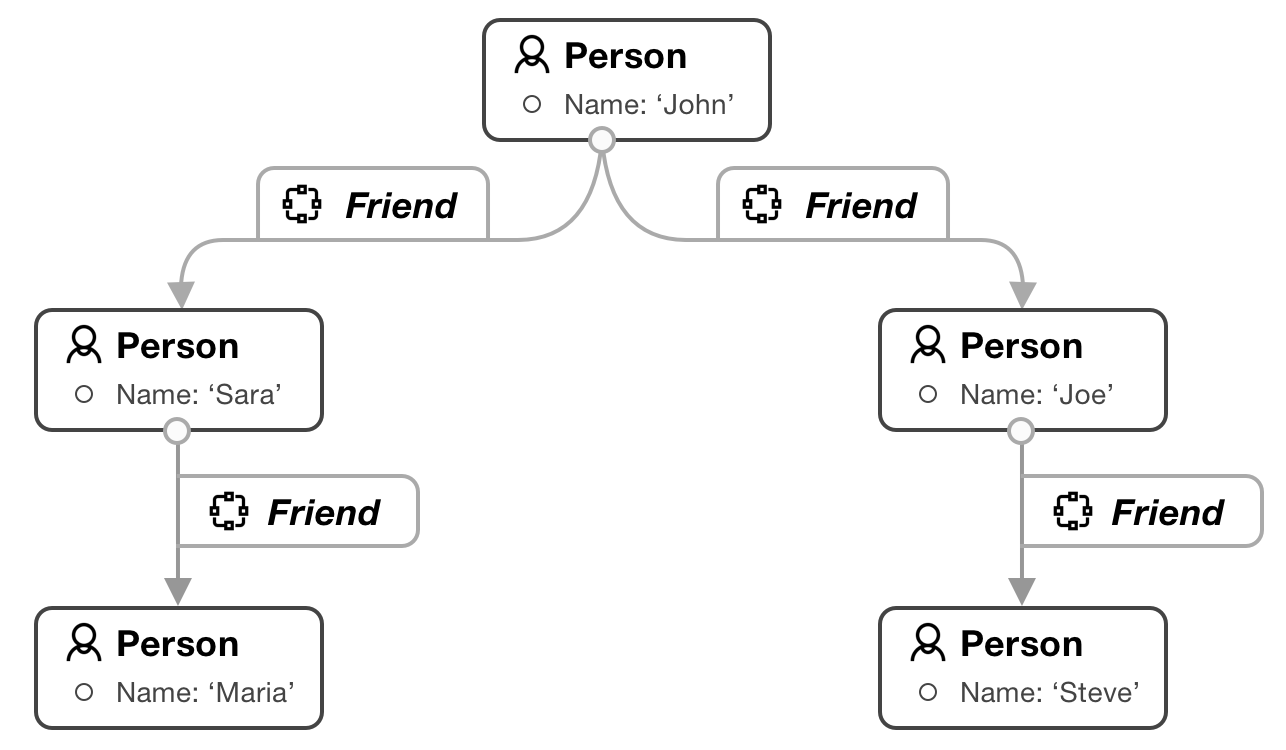
\includegraphics[scale=0.3]{figures/graph_cypher.png}
  \caption{Example graph with friendship relationships. Based on~\cite{neo4j_website}}
  \label{fig:graph_cypher}
\end{figure}

For example, we can build a Cypher query to be evaluated on the graph illustrated in \autoref{fig:graph_cypher} with using \textsf{Person} node and \textsf{Friend} edge labels.
When evaluated on this graph, the query in \autoref{lst:cypher_example} finds the \textsf{User} pairs ``John'' and ``Sara'' along with ``Joe'' and ''Steve''.

\begin{lstlisting}[language=Cypher,frame=single,label={lst:cypher_example},caption={Example query in Cypher}]
MATCH (user)-[:FRIEND]->(friend)
WHERE user.name IN ['Joe', 'John', 'Sara'] 
AND friend.name =~ 'S.*'
RETURN user.name, friend.name
\end{lstlisting}

\subsection{TigerGraph}

TigerGraph is a native parallel graph database system, built on the massively parallel computation of queries and analytics~\cite{tigergraph_website}.
The storage is designed to organize the graph nodes, edges, and their properties to be easily accessible by an engine that computes queries and analytics in massively parallel processing (MPP) fashion.
The system has been reported to provide strong scale-up and scale-out performance.
TigerGraph has the following main features~\cite{DBLP:journals/corr/abs-1901-08248}:

\begin{itemize}
  \item \textbf{A Native Distributed Graph:}
  While many graph database systems are built on a storage architecture that is a wrapper on top of a more generic NoSQL data store,
  TigerGraph developed its native database solution.
  This technology eliminates the double performance penalty with the virtual layer; in contrast, it enables the structure optimized for graph operations. 
  \item \textbf{Compact Storage with Fast Access:}
  TigerGraph stores the data in in-memory and disk storage in the enterprise edition.
  Users can configure the in-memory size, how much memory will be used for holding the graph.
  Data is stored in encoded and compressed formats.
  Compression factors vary from $2\times$ to $10\times$ based on the graph structure and data type.
  The encoding is homomorphic, so the decompression is used during data representation.
  During the data updates and computation processes, the decompression is not used.
  The database supports the indexing capability over the hash indices, which helps the system keep lookup performance constant while the graph grows in size.
  \item \textbf{Parallelism and Shared Values:}
  TigerGraph is designed to execute the queries in parallel fashion, supports massively parallel processing (MPP) in all aspects.
  The nature of graph traversals to follow the edges over connected nodes and fits for parallel/multithreaded execution.
  For example, in the breadth-first search algorithm developer needs to assign a temporary variable to each visited node and keeps tracking of these visits.
  This method should be implemented manually in the low-level languages, but it is possible to write even more complex graph traversals in a few lines of code using TigerGraph’s high-level query language.
  \item \textbf{Storage and Processing Engines Written in C\texttt{++}:}
  The storage and processing engines are developed in C\texttt{++.} 
  This enables the low-level memory management methods more accessible to the system.
  In alternative systems that are built on the JVM (Java Virtual Machine), it is much difficult for the system developer to handle the memory usage efficiently.
  \item \textbf{Automatic Partitioning:}
  In most cases, the essential database criteria in modern applications are scalability support; storing all data in one server is economically more expensive.
  TigerGraph partitions the graph data automatically across a server cluster.
  The hash index holds the information about node data and server location in a cluster.
  The edges and connected nodes are stored on the same server.
  \item \textbf{Distributed Computing:}
  TigerGraph computes the queries across the servers in a distributed model that increases the performance significantly.
  In distributed query mode, all servers are involved in the process; each server contributes own output or use the output from others on an as-needed basis.
  \item \textbf{Programming Abstraction: an MPP Computation Model:}
  TigerGraph offers the low-lever programming abstraction over the two classical graph programming paradigms of \textit{think-like-a-vertex} and \textit{think-like-an-edge}.
  In the user-defined programs, the nodes and edges are used as a parallel unit of storage and computation in a massively parallel computational mesh.
  \item \textbf{GSQL, a High-Level Graph Query Language:}
  GSQL is a high-level query language compatible with SQL syntax and Bulk-Synchronous Processing (BSP) terms.
  The queries are modelled in mostly \texttt{SELECT-FROM-WHERE} structure, like in SQL.
  Newly introduced accumulator clause \texttt{ACCUM} aggregates the outputs by parallel computation threads.
  GSQL is compatible with SQL, and MPP-aware interpretations make it easy to build queries by NoSQL developers.
  An example of GSQL queries will be discussed later in \autoref{sec:static_tigergrap_implementation}.
\end{itemize}

\subsection{Oracle PGX}

Oracle PGX is a scalable distributed pattern matching graph engine for large property graphs and introduced to the community in recent years~\cite{pgx_website}.
The engine evaluates the pattern matching queries using asynchronous depth-first traversal in parallel execution mode. 
PGX supports the PGQL~\cite{pgql_website}, an elegant SQL-like graph query language.
For example, in the query in \autoref{lst:pgx_query_example} return return all $a$ nodes with \texttt{age} more than 18 paired with their friends $b$.

\begin{lstlisting}[language=Cypher,frame=single,label={lst:pgx_query_example},caption={Example query in PGX. Based on~\cite{DBLP:conf/grades/RothTHCPMH17}}]
SELECT a, b WHERE (a WITH age > 18)-[:friend]->(b)
\end{lstlisting}

Oracle PGX accepts the PGQL queries as input and has four processing steps~\cite{DBLP:conf/grades/RothTHCPMH17}:

\begin{enumerate}
  \item PGX compiles the PGQL into a query plan using the query compiler\footnote{\url{https://pgql-lang.org/}}
  \item The system distributes the query plan to be evaluated by the distributed graph
  \item The engine translates the distributed query plan into an execution plan for every stage.
  A regular stage processes a single vertex, however, an inspection stage re-visits the processed vertices.
  Each stage constructs an advanced depth-first traversal sequence, and has dedicated components process the data (will be discussed in the following paragraph).
  \item PGX compiles the execution plan into memory and launches the computation.
  The runtime consists of multiple workers per machine, initialized by the task manager during system boot time.
  Computation commands are defined as tasks and placed in the task queues.
  Task queue manages the asynchronous operations to be computed.
  Some tasks can wait for another task to be completed in order to get the output as their input variable.
\end{enumerate}

Components are used in the stages~\cite{DBLP:conf/grades/RothTHCPMH17}:

\begin{itemize}
  \item \textbf{Vertex function:}
  The vertex function applies the PGQL vertex filters and builds the stage output context parts related to vertex properties.
  \item \textbf{Hop engine:}
  The hop engine orchestrates the traversal computations in vertices.
  There are several hop engine types that implement following traversal patterns:
  \begin{itemize}
    \item \textit{Vertices:}
    Hop to one or more vertices.
    Previously mentioned inspection stages are configured by this hop engine to hop one vertex.
    \item \textit{Out neighbors:}
    Hop to the connected neighbors from the current vertex.
    For example, in \texttt{(a) -[]-> (b)} the stage of \texttt{a} is assumed to have appeared before the one of \texttt{b}.
    \item \textit{In neighbors:}
    Hop into the incoming neighbors from the current vertex.
    For example, in \texttt{(a) <-[]- (b)} the stage of \texttt{a} is assumed to have appeared before the one of \texttt{b}.
    \item \textit{Common neighbors:}
    Hop to the common neighbors of two vertices. 
    For example, in \texttt{(a) -[]-> (b) <-[]- (c)} the stage of \texttt{b} is located between the stages of \texttt{a} and \texttt{c}.
    \item \textit{Output:}
    The last hop engine in a query passes the current stage's output to the collected global output.
  \end{itemize}
  \item \textbf{Message Manager:}
  The message manager handles the message transactions in cooperation with worker threads.
  Message types include both acknowledgment and work messages.
  There is one message manager per stage and multiple outgoing slots per worker.
  Outgoing messages are delivered to the next stage, while incoming messages are passed to the idle workers and computation units.
  The manager blocks the current stage computation if worker queues are full and cannot send a message over a thread.
  The message manager prevents the workers to get assigned for additional computations if they are already fully busy.
  \item \textbf{Flow Control Manager:}
  The flow control manager arranges the memory resources of each stage based on unprocessed messages in order to complete the computation.
  Manager can delay the messages intentionally to protect the machines from overload.
  Users can configure the memory limits for each machine.
\end{itemize}
